\documentclass[11pt,a4paper]{article}
\usepackage[margin=24mm,headheight=15pt]{geometry}
\usepackage[T1]{fontenc}
\usepackage{lmodern,microtype,amsmath,amssymb,booktabs,tabularx,array,graphicx,xcolor,fancyhdr,listings,enumitem}
\usepackage[colorlinks=true,linkcolor=black,urlcolor=blue,citecolor=black]{hyperref}
\hypersetup{pdftitle={Transient Thermal Analysis of Automotive Disc Brakes Using FEA},pdfauthor={Yug Bhushan}}
\setlength{\parskip}{6pt}\setlength{\parindent}{0pt}\setlist{nosep,leftmargin=1.5em}\renewcommand{\arraystretch}{1.2}
\pagestyle{fancy}\fancyhf{}\fancyhead[L]{\small Transient Thermal Analysis of Disc Brakes}\fancyhead[R]{\small Yug Bhushan}\fancyfoot[C]{\thepage}
\lstset{language=Python,basicstyle=\ttfamily\scriptsize,breaklines=true,columns=fullflexible,keepspaces=true,showstringspaces=false,frame=single,rulecolor=\color{black!20},numbers=left,numberstyle=\tiny\color{black!50},numbersep=7pt,xleftmargin=10pt,framexleftmargin=5pt}
\newcommand{\sectionpage}[1]{\clearpage\section{#1}}
\begin{document}
\begin{titlepage}\centering\vspace*{22mm}
{\Large\scshape Term Paper\par}\vspace{16mm}
{\huge\bfseries Transient Thermal Analysis of Automotive Disc Brakes Using FEA\par}\vspace{10mm}
{\large Conduction, Convection, Radiation,\\and a Comparison of Rotor Materials\par}\vspace{24mm}
{\Large Yug Bhushan\par}\vspace{3mm}{\large 2025CH71601\par}\vspace{7mm}
Department of Chemical Engineering\\Indian Institute of Technology Delhi
\vfill{\large Project period: February 2026\par}\vspace{12mm}
\end{titlepage}

\section*{Abstract}\addcontentsline{toc}{section}{Abstract}
During braking, a vehicle's kinetic energy is converted into heat at the rotor--pad interface. The resulting temperature field depends on the braking history, heat partition, rotor geometry, material properties, and heat loss to the surroundings. This paper develops a transient finite element framework for studying this process, with particular attention to comparing gray cast iron and a silicon-carbide-containing carbon-ceramic rotor. The model includes internal conduction, convection, and surface radiation. The braking load is derived from an energy balance, and the weak formulation, time integration, and numerical verification requirements are presented.

The supplied project summary states that a transient model was built in COMSOL and that the two material systems were compared under panic braking, with superior thermal stability reported for the ceramic option. The original COMSOL model, property tables, geometry, and numerical outputs were not provided. Consequently, no original peak temperatures, temperature contours, or material-specific convergence results are invented here. Carbon-ceramic composite properties are distinguished from those of monolithic silicon carbide, and lower operating temperature is distinguished from the ability to retain performance at elevated temperature.

To make the numerical discussion concrete, an independently constructed one-dimensional finite element verification problem is solved using explicitly assumed inputs. It reproduces the energy balance of a symmetrically heated slab and supplies separate mesh and time-step refinement calculations. For its finest tested discretization, the illustrative surface peak is approximately 378.01 K. This value belongs only to the verification problem, not to either original COMSOL material case. A Python appendix and a documented COMSOL setup protocol support reproduction and future completion of the original material comparison.

\textbf{Keywords:} disc brake; transient heat transfer; finite element analysis; COMSOL; gray cast iron; carbon-ceramic composite; thermal verification.

\subsection*{Scope and evidence}
The title, project period, software, heat-transfer mechanisms, and reported qualitative material comparison follow the supplied project summary. Model parameters and one-dimensional results introduced here are explicitly illustrative. COMSOL has not been executed for this manuscript, and the Python verification model does not reproduce a three-dimensional moving contact patch.

\clearpage\begingroup\small\tableofcontents\endgroup

\clearpage\section*{Nomenclature}\addcontentsline{toc}{section}{Nomenclature}
\begin{tabularx}{\textwidth}{@{}lXl@{}}\toprule
Symbol & Meaning & Unit\\\midrule
$m_v$ & Vehicle mass & kg\\
$v,a$ & Vehicle speed and deceleration magnitude & m s$^{-1}$, m s$^{-2}$\\
$t_b$ & Braking duration & s\\
$f_a,N_r$ & Axle energy fraction and rotors on that axle & --\\
$\eta_r$ & Fraction of allocated frictional heat entering a rotor & --\\
$P_r,Q_r$ & Rotor heating power and total energy input & W, J\\
$q_{\mathrm{in}}''$ & Applied inward heat flux & W m$^{-2}$\\
$r_o,r_i,b$ & Rotor outer radius, inner radius, and thickness & m\\
$T,T_0$ & Temperature and initial temperature & K\\
$T_\infty,T_s$ & Air and radiative-surroundings temperatures & K\\
$\rho,c_p$ & Density and specific heat capacity & kg m$^{-3}$, J kg$^{-1}$ K$^{-1}$\\
$\mathbf k,k$ & Conductivity tensor and isotropic conductivity & W m$^{-1}$ K$^{-1}$\\
$\alpha$ & Thermal diffusivity, $k/(\rho c_p)$ & m$^2$ s$^{-1}$\\
$h,\epsilon$ & Convection coefficient and emissivity & W m$^{-2}$ K$^{-1}$, --\\
$\sigma$ & Stefan--Boltzmann constant & W m$^{-2}$ K$^{-4}$\\
$\mathbf u$ & Local material velocity in a spatial frame & m s$^{-1}$\\
$M,K$ & Finite element heat-capacity and conduction matrices & model dependent\\
$E_{\mathrm{in}},E_{\mathrm{out}}$ & Integrated energy input and loss & J\\
Bi, Fo & Biot and Fourier numbers & --\\\bottomrule
\end{tabularx}

\subsection*{Temperature and sign conventions}
All radiation expressions use absolute temperature in kelvin. A temperature difference of one kelvin equals one degree Celsius, but absolute temperatures are not interchangeable in a fourth-power radiation law. The boundary normal points outward, and $q_{\mathrm{in}}''$ is positive when energy enters the rotor. Heat flux density in W m$^{-2}$ must be distinguished from total power in W and from energy in J.

\sectionpage{Introduction and Engineering Context}
\subsection{Braking as a transient heat-transfer problem}
A brake converts mechanical energy into thermal energy over a short contact interval. Heat initially enters a limited surface region, spreads through the rotor, and is subsequently transferred to the pad, mounting system, and surrounding air. A single average temperature does not describe the contact-region peak or the through-thickness gradient.

A transient thermal model is therefore useful for identifying the time and location of a temperature maximum and the rate of cooling after release. COMSOL's public disc-brake example demonstrates this class of problem with conduction, frictional heating, and external losses \cite{comsol}. Its numerical results belong to that example and are not adopted as results of the present project.

The governing principles are directly connected to chemical engineering transport phenomena: an unsteady energy balance, constitutive heat-conduction laws, and heat-transfer boundary conditions. Finite element analysis supplies a numerical solution when geometry and boundary loading make a closed-form solution impractical.

\subsection{Why material comparison requires a precise basis}
Thermal conductivity controls spatial heat spreading, while density and heat capacity determine thermal storage. Surface emissivity affects radiation, and the pad--rotor contact affects how frictional heat is shared. A material may resist thermal degradation while reaching a higher temperature than another rotor of equal geometry. Conversely, lower peak temperature does not alone establish better friction stability or fatigue resistance.

For a useful comparison, the braking event and the design constraints must be stated. Equal geometry, equal mass, and independently optimized geometry are different studies. A rotor that is lighter at the same dimensions also has a different total heat capacity. Ignoring this change can lead to an incorrect explanation of the temperature response.

\subsection{Objectives}
This paper aims to derive the braking heat input, formulate the transient thermal problem, explain finite element discretization and COMSOL implementation, and define the evidence needed for a fair gray-cast-iron versus carbon-ceramic comparison. A separate numerical verification example demonstrates energy conservation and discretization sensitivity without inventing original simulation results.

The work concerns thermal response. Thermal stress, friction coefficient degradation, wear, cracking, and stopping-distance predictions require additional constitutive information or coupled analyses and are not inferred from temperature contours alone.

\sectionpage{Braking Energy and Surface Heat Input}
\subsection{Vehicle energy balance}
Neglecting aerodynamic drag, rolling resistance, road grade, and rotational inertia for a first approximation, the kinetic energy removed between speeds $v_0$ and $v_f$ is
\begin{equation}
E_b=\frac12m_v(v_0^2-v_f^2).
\end{equation}
If $v(t)=v_0-at$ during constant-magnitude deceleration, then
\begin{equation}
t_b=(v_0-v_f)/a,\qquad P_b(t)=-\frac{d}{dt}\left(\frac12m_vv^2\right)=m_vav(t).
\end{equation}
The braking power decreases with speed and vanishes on release. A prescribed constant heat flux of the same duration would represent a different loading history unless its total energy and intended approximation are explicitly matched.

A more complete vehicle model can add wheel rotational energy and subtract non-brake losses. Those contributions should be introduced through a consistent system energy balance rather than through arbitrary correction factors.

\subsection{Allocation to one rotor}
Let $f_a$ be the fraction dissipated at the modeled axle, $N_r$ the number of rotors on that axle, and $\eta_r$ the fraction of its allocated frictional heat entering one rotor. Then
\begin{equation}
P_r(t)=\eta_r\frac{f_a}{N_r}P_b(t),\qquad
Q_r=\eta_r\frac{f_a}{N_r}E_b.
\end{equation}
The pad receives the remaining contact heat in a two-body description. A rotor-only thermal model can instead prescribe $\eta_r$ explicitly, provided it is justified or varied in a sensitivity study. COMSOL's thermal-contact formulation also supports partitioning friction heat between contacting bodies \cite{contact}.

For a total heated area $A_h$ on the rotor,
\begin{equation}
q_{\mathrm{in}}''(t)=P_r(t)/A_h.
\end{equation}
If both full annular faces are uniformly heated, $A_h=2\pi(r_o^2-r_i^2)$. If a localized pad footprint is heated, its actual area and moving coverage are used instead. Applying the full power independently to both faces would double the intended energy.

\subsection{Friction-based alternative}
When pressure $p$ and sliding speed $v_s$ are specified, the local frictional generation is $q_f''=\mu p v_s$. This is the total contact generation before partitioning. A simulation should use either a mechanically consistent friction specification or an energy-derived thermal load; it should not add both descriptions of the same dissipation.

\sectionpage{Governing Thermal Equations}
\subsection{Conduction and storage}
For a rotor described in a material frame, the heat equation is
\begin{equation}\label{eq:heat}
\rho c_p(T)\frac{\partial T}{\partial t}=\nabla\cdot(\mathbf k(T)\nabla T)+\dot q_v.
\end{equation}
The volumetric source $\dot q_v$ is zero when frictional heating is represented entirely at the surface. For an isotropic material, $\mathbf k=kI$. For a composite, radial, circumferential, and through-thickness conductivities may differ and must be aligned with the material orientation.

The initial condition is
\begin{equation}
T(\mathbf x,0)=T_0(\mathbf x).
\end{equation}
Assuming a uniform ambient initial state is a useful reference case. A repeated-braking study instead begins each event from the temperature field remaining after the preceding event.

\subsection{Convection, radiation, and inward heating}
With outward normal $\mathbf n$ and conductive flux $-\mathbf k\nabla T$, the exposed-surface boundary condition is
\begin{equation}\label{eq:bc}
\mathbf n\cdot(-\mathbf k\nabla T)
=h(T-T_\infty)+\epsilon\sigma(T^4-T_s^4)-q_{\mathrm{in}}''.
\end{equation}
This sign convention gives positive outward heat loss when the rotor is hotter than the air or surroundings. The source term may be zero on unheated surfaces. Contact-covered regions should not automatically receive the same external convection as surfaces directly exposed to airflow.

A convection coefficient can depend on position, time, vehicle speed, rotor rotation, and ventilation geometry. A constant $h$ is a declared simplification. It should not be treated as a universal property of the rotor material. Surface radiation is nonlinear, and emissivity depends on the actual surface condition.

\subsection{Contact and mounting conditions}
A simplified pad contact can use a thermal conductance $H_c$ with heat exchange proportional to $T_r-T_p$. A hub boundary may be insulated, assigned a contact conductance, or coupled to an explicit mounting domain. Prescribing a fixed ambient hub temperature can impose a strong artificial sink and should be justified.

The assumptions chosen for contact and hub heat removal must be identical across the material comparison unless the aim is to study their differences. When the pad is omitted, the chosen heat-partition fraction and thermal boundary conditions carry the effect of that simplification.

\clearpage
\subsection{Rotation and reference-frame consistency}
In a stationary spatial frame, rotating material transports stored heat through the field. For rigid rotation about the $z$ axis,
\begin{equation}
\mathbf u=(-\omega y,\omega x,0),\qquad
\rho c_p\left(\frac{\partial T}{\partial t}+\mathbf u\cdot\nabla T\right)
=\nabla\cdot(\mathbf k\nabla T)+\dot q_v.
\end{equation}
An alternative uses material coordinates attached to the rotor and moves the pad heating footprint relative to those coordinates. The source trajectory and material-motion terms must represent one consistent frame transformation. Moving a source and independently adding an inconsistent rotation term can misrepresent the relative motion.

An axisymmetric or full-annulus heat load averages the circumferential variation. It can be useful for mean heating and energy checks, but it cannot reproduce localized moving contact hotspots. The one-dimensional verification problem used later applies this averaging deliberately and contains no rotational advection term.

\subsection{Integrated energy balance}
For constant density and specific heat, rotor energy relative to $T_0$ is
\begin{equation}
U(t)=\int_\Omega\rho c_p[T(\mathbf x,t)-T_0]\,dV.
\end{equation}
With temperature-dependent heat capacity, use specific enthalpy,
\begin{equation}
U(t)=\int_\Omega\rho\int_{T_0}^{T(\mathbf x,t)}c_p(\theta)\,d\theta\,dV,
\end{equation}
under the small-deformation, constant-reference-density approximation. For a rotor-only model, the energy balance is
\begin{equation}
U(t)-U(0)=E_{\mathrm{in}}-E_{\mathrm{conv}}-E_{\mathrm{rad}}-E_{\mathrm{hub}}-E_{\mathrm{contact}},
\end{equation}
where each outflow is signed outward and integrated over time. If the prescribed inward input is already the net heat entering the rotor after pad partition, the excluded pad fraction is not subtracted a second time.

\subsection{Characteristic time and temperature scales}
Thermal diffusivity is $\alpha=k/(\rho c_p)$. Heat diffusion over distance $L_c$ occurs on a scale $t_d\sim L_c^2/\alpha$. The Fourier number $\mathrm{Fo}=\alpha t/L_c^2$ compares elapsed time with this scale. The Biot number $\mathrm{Bi}=hL_c/k$ compares external convection with conduction resistance. A small convection Biot number alone does not prove uniform temperature during intense localized surface heating; the heat-input distribution and transient diffusion must also be considered.

\sectionpage{Rotor Materials and a Fair Comparison}
\subsection{Gray cast iron and carbon-ceramic terminology}
The project describes a comparison between gray cast iron and a carbon-ceramic material labelled SiC. Commercial automotive carbon-ceramic rotors are composite systems: for example, Brembo SGL lists carbon, silicon, and silicon-carbide constituents and distinguishes the core from the friction layer \cite{composite}. Pure, monolithic silicon-carbide properties should therefore not be substituted for a composite rotor without explaining that approximation.

The material specification should identify the gray-cast-iron grade and the ceramic composite architecture, porosity, fiber arrangement, and surface layer. If only a generic library material was used in the original model, the report should state that explicitly rather than assign properties from a different product.

\subsection{Properties controlling thermal response}
\begin{tabularx}{\textwidth}{@{}lX@{}}\toprule
Property & Role in the comparison\\\midrule
$\rho c_p$ & Volumetric thermal storage; controls mean rise for fixed volume and input energy.\\
$k$ or $\mathbf k$ & Conductive spreading and the magnitude of internal temperature gradients.\\
$\alpha$ & Rate of diffusion relative to the braking duration.\\
$\epsilon$ & Radiative exchange with the surroundings.\\
Thermal expansion & Needed for deformation and thermal-stress interpretation, not for a conduction-only solution.\\
Friction and stability data & Needed to evaluate fading or retained braking behavior, beyond temperature alone.\\\bottomrule
\end{tabularx}

A higher conductivity can reduce a localized surface rise by distributing energy into more material. A higher specific heat can lower temperature rise for equal mass. For equal geometry, the relevant storage is $\rho c_pV$, so density must also be considered. None of these isolated properties establishes a universal material ranking.

\subsection{Comparison protocols}
An equal-geometry study holds dimensions, contact area, and load history fixed and changes material data. An equal-mass study changes geometry or volume and therefore changes conduction paths and cooling area. An application-specific optimization can change both material and shape, but should be presented as a design comparison rather than an isolated material test.

Use the same input energy, initial state, air conditions, contact assumptions, and numerical tolerances when isolating material effects. If heat partition is recalculated from material properties, report it for each case because it changes the rotor input itself. A fixed-partition comparison and a contact-coupled comparison answer different questions.

\sectionpage{Finite Element Formulation and Time Integration}
\subsection{Weak formulation}
For a nonmoving material-frame problem, multiply Equation \eqref{eq:heat} by a test function $w$ and integrate over the rotor. Applying integration by parts and Equation \eqref{eq:bc} gives
\begin{align}
&\int_\Omega w\rho c_p\dot T\,dV
+\int_\Omega\nabla w\cdot\mathbf k\nabla T\,dV\nonumber\\
&+\int_{\Gamma}wh(T-T_\infty)\,dA
+\int_{\Gamma}w\epsilon\sigma(T^4-T_s^4)\,dA\nonumber\\
&=\int_\Omega w\dot q_v\,dV+\int_{\Gamma}wq_{\mathrm{in}}''\,dA.
\end{align}
Boundary integrals are taken only over the surfaces to which their respective conditions apply. Contact or fixed-temperature terms require the corresponding additions or constraints.

Approximating $T_h=\sum_jN_jT_j$ and choosing Galerkin test functions gives
\begin{equation}
M(\mathbf T)\dot{\mathbf T}+K(\mathbf T)\mathbf T+
\mathbf g_{\mathrm{conv}}(\mathbf T)+\mathbf g_{\mathrm{rad}}(\mathbf T)=\mathbf f(t),
\end{equation}
where the element contributions include
\begin{equation}
M_{ij}=\int_{\Omega_e}\rho c_pN_iN_j\,dV,\qquad
K_{ij}=\int_{\Omega_e}\nabla N_i\cdot\mathbf k\nabla N_j\,dV.
\end{equation}
For constant $h$, the convection matrix contains $\int_\Gamma hN_iN_j\,dA$. The ambient temperature supplies a boundary load. Radiation remains nonlinear.

\subsection{Implicit time stepping}
A backward-Euler step has the residual
\begin{equation}
\mathbf R(\mathbf T^{n+1})=
\frac{M}{\Delta t}(\mathbf T^{n+1}-\mathbf T^n)
+K\mathbf T^{n+1}+\mathbf g(\mathbf T^{n+1})-\mathbf f^{n+1}.
\end{equation}
A Newton update solves $J\Delta\mathbf T=-\mathbf R$, then updates the trial temperature. For a radiating boundary, the local tangent contains $4\epsilon\sigma T^3$. Temperature-dependent material properties introduce further nonlinearities.

The appendix uses constant properties, a consistent heat-capacity matrix, implicit conduction and surface losses, and midpoint sampling of the prescribed heat input. It uses Newton iteration for radiation. It is an illustrative independent implementation, not a description of an undocumented original COMSOL solver configuration.

\clearpage
\subsection{Mesh design and localized loading}
In a three-dimensional rotor model, use local refinement near the pad contact track, outer and inner edges, geometric transitions, and thin sections. Several elements through thickness may be needed to resolve a surface-heating gradient. A visually smooth contour is not evidence of mesh independence.

A localized source with a sharp artificial edge can make the reported point maximum sensitive to geometry, source smoothing, and element size. The load footprint should reflect the physical approximation being studied. Compare peak temperature, a representative probe trace, and volume-mean temperature during refinement rather than relying on one color scale.

\subsection{Output times and internal solver steps}
Requested plotting times and the solver's internal time steps are different quantities. Dense output can interpolate a solution without resolving a rapidly changing heat input accurately. The maximum internal step should be limited relative to the braking duration and, for moving contact, the time for the heat source to cross a mesh element or probe region.

A piecewise load that starts or stops abruptly needs event handling or a suitably resolved transition. If smoothing is used, integrate the resulting load to verify that its energy remains the intended value. A smoother source with a different area under its curve is a different braking event.

\subsection{Verification hierarchy}
Verification asks whether the chosen equations have been solved accurately. It includes an energy audit, mesh refinement, time-step refinement, and comparison with a simplified problem of known behavior. COMSOL's documentation recommends resolving the model on successively finer meshes and comparing relevant results \cite{mesh}.

Validation asks whether the equations and parameters adequately represent a physical brake. It requires independent measurements, such as dynamometer thermocouple or infrared observations with their own uncertainty and response characteristics. Agreement between two meshes or two simulation programs is not experimental validation.

\subsection{Thermal stress as an extension}
Temperature differences can drive differential expansion, but a thermal model does not directly compute stress. A subsequent structural calculation requires the thermal expansion coefficient, elastic or inelastic properties, constraints, and possibly anisotropy. Inferring a crack probability from a maximum temperature alone is unsupported without an appropriate failure model and material data.

\sectionpage{Proposed COMSOL Modeling Procedure}
\subsection{Geometry, parameters, and materials}
Create a three-dimensional rotor geometry that represents the actual modeled disc and pad configuration. Record the radii, thickness, vent geometry, pad footprint, and mounting representation. Named selections for friction tracks, exposed faces, rim, hub, and contact boundaries help keep both material cases consistent.

Define unit-bearing parameters for vehicle mass, speed, braking duration, axle fraction, rotor allocation, and thermal partition. Enter sourced material data as functions of temperature where available. Assign the material to the correct rotor domains and verify the tensor orientation if conductivity is anisotropic. The numerical values in Section 8 are demonstration inputs, not recovered COMSOL settings.

\subsection{Physics and boundary conditions}
Use a transient heat-transfer formulation appropriate for the chosen frame. The official COMSOL brake example uses a three-dimensional heat-transfer model and accounts for rotational material motion \cite{comsol}. A rotor-only reconstruction can use prescribed inward heating; an explicit rotor--pad model can instead use frictional thermal contact.

Apply convection and surface-to-ambient radiation to the exposed selections, with consistent air and surroundings temperatures. Define hub and pad contact behavior separately. Check that no duplicate boundary source adds the same frictional energy twice. For a rotor-only approach, an area integral of the inward heat flux should recover $P_r(t)$.

\subsection{Study and postprocessing}
Run a Time Dependent study through braking and sufficient release time to characterize cooling. Use the same time-control and tolerance protocol for both material cases. Repeat on refined meshes and smaller maximum steps before comparing small differences between peak temperatures.

Extract the following quantities for each case: maximum rotor temperature versus time; its location and time; volume-mean temperature; selected radial and through-thickness probe traces; and integrated heat input, storage, and losses. Plot material cases with identical units, scales, and evaluation times. A maximum extracted from a sparse set of saved times may miss a short contact-region peak.

\subsection{Reproducible records}
Retain the COMSOL version, model file, parameter table, material references, selection definitions, element count, solver settings, and exported numerical tables. A screenshot alone cannot establish the load normalization, material identity, or convergence. The source archive accompanying this paper contains documentation and a Python verification example; it does not contain an original or newly generated COMSOL \texttt{.mph} model.

\sectionpage{Verification Criteria and Sensitivity Analysis}
\subsection{Conservation and normalization}
Integrate the prescribed power and confirm that it matches the allocated braking energy. Independently integrate the surface source on the selected boundaries. This detects incorrect face counts, area conversions, and power-versus-flux confusion before interpreting a temperature field.

For $E_{\mathrm{in}}>0$, a useful conservation residual is
\begin{equation}
\delta_E(t)=\frac{|E_{\mathrm{in}}(t)-E_{\mathrm{out}}(t)-[U(t)-U(0)]|}
{E_{\mathrm{in}}(t)}.
\end{equation}
At very early times the denominator is small, so a run-wide normalization by the final input energy may be more stable. The appendix reports the maximum absolute energy mismatch divided by total input energy. A very small value indicates discrete conservation; it does not prove spatial accuracy or physical realism.

\subsection{Independent discretization studies}
To study spatial error, refine the mesh with the time discretization held fixed. To study temporal error, decrease the time step with a sufficiently resolved mesh held fixed. Changing both simultaneously can show improvement but does not identify which source of error dominates.

Track temperature rise above the initial state when expressing relative changes; dividing by absolute kelvin temperature can understate error in the predicted rise. A practical tolerance should be selected according to the study's purpose and expected material differences, rather than assuming that an arbitrary percentage is universally sufficient.

\subsection{Parameters worth varying}
Heat-partition fraction, convection coefficient, pad footprint, material conductivity, volumetric heat capacity, emissivity, and hub contact can all affect the predicted response. Change one parameter at a time for an initial sensitivity study, then consider interactions if the design decision depends on them. Keep total braking energy fixed when investigating a geometric redistribution of the same load.

A comparison whose temperature difference is smaller than the uncertainty caused by heat partition or material properties should be presented cautiously. Sensitivity to uncertain boundary conditions is a different issue from mesh convergence and cannot be removed merely by increasing the element count.

\subsection{Limits of a prescribed-load model}
Prescribing a deceleration-derived heat input assumes a braking trajectory rather than predicting it. A temperature-dependent friction coefficient cannot independently alter that trajectory unless the mechanical braking model is coupled consistently. Similarly, prescribed convection does not resolve ventilation airflow. These are deliberate modeling choices that define the scope of the thermal calculation.

\sectionpage{Illustrative Calculations and Independent FEA Example}
\subsection{Assumed braking event and geometry}
The following values are deliberately selected for demonstration. They are not the original project's parameters or a certified material dataset.
\begin{table}[h!]\centering\small
\begin{tabularx}{\textwidth}{@{}lXl@{}}\toprule
Quantity & Assumed value & Unit\\\midrule
Vehicle mass, initial/final speed & 1500; 25 / 0 & kg; m s$^{-1}$\\
Deceleration magnitude & 8 & m s$^{-2}$\\
Axle fraction; rotors on axle & 0.70; 2 & --\\
Rotor heat fraction & 0.90 & --\\
Outer / inner radius; thickness & 0.14 / 0.07; 0.013 & m\\
Reference density / heat capacity & 7200 / 500 & kg m$^{-3}$ / J kg$^{-1}$ K$^{-1}$\\
Reference conductivity & 50 & W m$^{-1}$ K$^{-1}$\\
Convection coefficient; emissivity & 50; 0.8 & W m$^{-2}$ K$^{-1}$; --\\
Initial, air, surroundings temperature & 300 & K\\\bottomrule
\end{tabularx}
\caption{Illustrative inputs. The reference properties do not establish either original material's identity.}
\end{table}

The braking duration and removed kinetic energy are
\begin{equation}
t_b=25/8=3.125\ \mathrm{s},\qquad E_b=\tfrac12(1500)(25^2)=468{,}750\ \mathrm{J}.
\end{equation}
One modeled rotor receives
\begin{equation}
Q_r=0.90\frac{0.70}{2}E_b=147{,}656.25\ \mathrm{J}.
\end{equation}
Its annular face area is 0.0461814 m$^2$, volume 0.000600358 m$^3$, and mass approximately 4.32258 kg. Total thermal capacity is 2161.29 J K$^{-1}$. The adiabatic uniform-temperature estimate is
\begin{equation}
\Delta T_{\mathrm{ad}}=Q_r/(\rho Vc_p)=68.3186\ \mathrm{K}.
\end{equation}
This is a bulk energy estimate, not an upper bound on local surface temperature. The initial rotor power is 94.5 kW and the initial flux on each of the two uniformly heated faces is approximately 1.02314 MW m$^{-2}$.

\clearpage
\subsection{Independent one-dimensional finite element problem}
A slab through the rotor thickness is modeled per unit annular face area. Equal heating on both faces permits use of a half-thickness domain $0\leq x\leq b/2$, with an insulated midplane and a heated, convecting, radiating outer surface. Radial and circumferential variations, edge losses, pad geometry, and hub conduction are excluded.

Linear elements use the consistent matrices
\begin{equation}
M_e=\frac{\rho c_p\ell_e}{6}\begin{bmatrix}2&1\\1&2\end{bmatrix},\qquad
K_e=\frac{k}{\ell_e}\begin{bmatrix}1&-1\\-1&1\end{bmatrix}.
\end{equation}
The heat flux decreases linearly during braking and is zero after 3.125 s. Conduction and losses are solved implicitly; the time grid includes the release instant explicitly. The Python implementation and figure are reproducible calculations for this manuscript, not exports from COMSOL.

\begin{figure}[h!]\centering
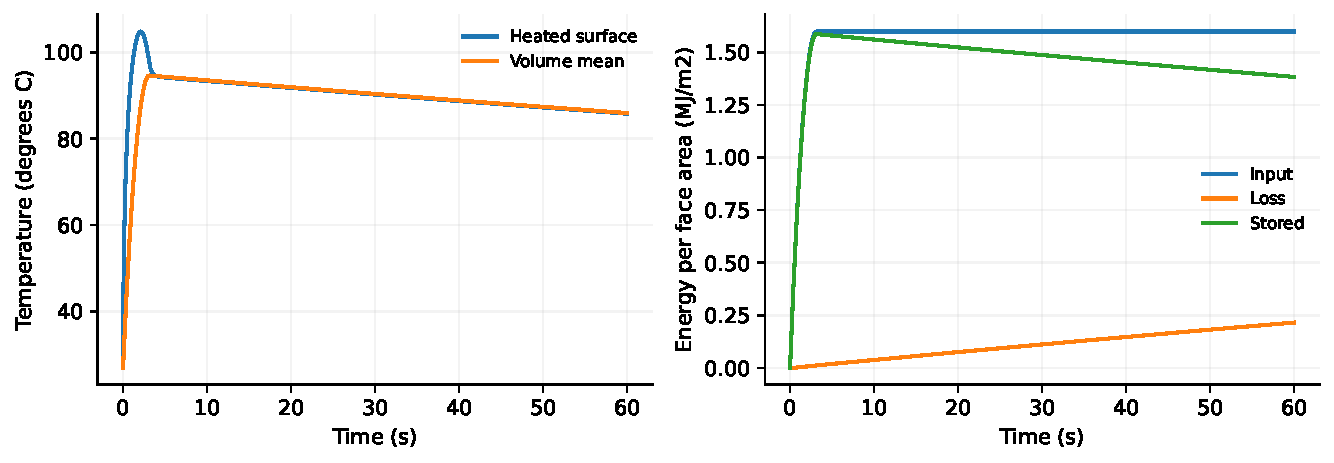
\includegraphics[width=\textwidth]{verification.pdf}
\caption{Independent illustrative one-dimensional FEA: surface/mean temperatures and energy per annular face area. The input equals stored energy plus losses to numerical precision.}
\end{figure}

For 40 elements and a nominal 0.025 s step, the computed surface peak is 378.0072 K (104.8572\,$^\circ$C) at 2.10 s. The mean temperature reaches approximately 367.8069 K at release. The surface peaks earlier because the applied power is decreasing while conduction and surface losses redistribute energy. At release, the mean rise is below the 68.3186 K adiabatic estimate because some heat has already escaped.

The half-thickness diffusion scale is about 3.042 s, comparable with the braking duration. The convection Biot number based on half thickness is only 0.0065, yet a transient surface-to-mean difference develops during heating. This illustrates why a small external-convection Biot number does not alone justify an isothermal rotor under prescribed surface loading.

\clearpage
\subsection{Independent mesh and time-step results}
\begin{table}[h!]\centering\small
\begin{tabular}{@{}lrrrr@{}}\toprule
Study & Elements & Nominal $\Delta t$ (s) & Surface peak (K) & Mean peak (K)\\\midrule
Mesh &10&0.025&377.9753&367.8073\\
Mesh &20&0.025&378.0008&367.8070\\
Mesh &40&0.025&378.0072&367.8069\\\midrule
Time &40&0.100&378.4934&367.8009\\
Time &40&0.050&378.1710&367.8049\\
Time &40&0.025&378.0072&367.8069\\\bottomrule
\end{tabular}
\caption{Calculated refinement results for the independent slab example only.}
\end{table}
At fixed nominal 0.025 s time step, refining 20 to 40 elements changes the surface peak by approximately 0.0064 K. At fixed 40 elements, decreasing the nominal step from 0.050 to 0.025 s changes it by approximately 0.1638 K. Temporal error is therefore more visible than the final mesh increment for these tested settings. These comparisons do not establish an exact continuum peak or justify assigning the same uncertainty to a moving three-dimensional hotspot.

The maximum energy mismatch normalized by total input remains below $2\times10^{-13}$ in these runs. This very small residual reflects conservation by the discrete equations with consistent quadrature of the time-discrete input and losses. The nonzero time-step effect despite a small energy residual shows that energy conservation alone is not an accuracy test.

\subsection{Capacity comparison without assigning a material winner}
For two rotors of equal volume receiving the same net heat, the adiabatic mean-rise ratio is
\begin{equation}
\frac{\Delta T_A}{\Delta T_B}=\frac{\rho_Bc_{p,B}}{\rho_Ac_{p,A}}.
\end{equation}
Thus, higher specific heat alone does not ensure a lower mean rise when density changes. For equal mass, the corresponding ratio depends on specific heat instead, but the changed geometry may alter local gradients and cooling.

No numerical carbon-ceramic property set is assigned in this paper because the original composite specification was not supplied. The independent reference calculation provides a check of mathematics and implementation; it cannot substantiate a gray-cast-iron versus composite ranking.

\sectionpage{Reported Project Outcome and Material Discussion}
\subsection{Evidence supplied by the project summary}
\begin{table}[h!]\centering\small
\begin{tabularx}{\textwidth}{@{}lX@{}}\toprule
Item & Supported statement and evidence limit\\\midrule
Software and study & A transient COMSOL FEA model is reported. The original model file and solver settings were not supplied.\\
Heat transfer & Conduction, convection, and radiation are reported as included. Boundary selections and parameter functions are not supplied.\\
Materials & Gray cast iron and a SiC-labelled carbon-ceramic option were compared. Grades, architecture, and property tables are not supplied.\\
Braking event & Panic braking is stated. Vehicle inputs, geometry, and heat partition are not supplied.\\
Reported conclusion & Superior thermal stability of the ceramic option is reported. Numerical peaks, gradients, and supporting stability criteria are not supplied.\\\bottomrule
\end{tabularx}
\caption{Project claims are attributed to the supplied description. The separate slab results are not original project outcomes.}
\end{table}

\subsection{Peak temperature and thermal stability}
A material comparison should report each rotor's peak temperature, the time and location of that peak, its mean temperature, and the thermal gradients under the declared loading. These values can establish differences in modeled thermal response. They do not by themselves quantify retained friction coefficient, wear resistance, thermal fatigue, or cracking.

The phrase superior thermal stability should be connected to an explicit criterion: for example, a smaller computed gradient under a fixed load, a lower modeled peak under a defined equal-geometry comparison, or experimentally supported retention of frictional behavior. Each is a different statement requiring different evidence.

\subsection{What completes the original comparison}
The original COMSOL model or exported data would permit insertion of material-specific property tables, common load and boundary definitions, temperature histories, contour plots with matching scales, and numerical refinement results. Contact heat partition should be reported for both cases. If the composite was represented by monolithic SiC properties, that approximation should be stated and its influence considered.

Until those records are available, the qualitative material conclusion remains the project's reported finding. No temperature reduction percentage, exact material peak, or claim of experimentally validated thermal stability is assigned here.

\sectionpage{Conclusions and Future Scope}
\subsection{Conclusions}
Transient disc-brake heating is governed by the competition between short-duration frictional input, internal conduction, thermal storage, and external heat loss. An energy-derived heat source provides a consistent link between a braking trajectory and the applied rotor load. Normalizing that load over the correct contact area and number of faces is essential.

A finite element model should retain a consistent reference frame, distinguish pad contact from exposed cooling surfaces, and verify energy conservation together with spatial and temporal accuracy. The independent slab calculation in this paper demonstrates that a well-conserved numerical solution can still have a measurable time-step effect on peak temperature.

The supplied project summary reports a COMSOL comparison of gray cast iron and a SiC-labelled carbon-ceramic rotor with superior thermal stability for the ceramic option. That result is preserved as reported, without inventing original temperatures or properties. A fair comparison requires the actual material specification and a clear definition of geometry, mass, heat partition, and stability criterion. Composite properties should not be assumed equal to those of monolithic SiC.

\subsection{Future work}
The next stage is to recover the original COMSOL model and numerical exports, then document a common comparison protocol. Material data should be temperature dependent where supported, and the composite conductivity orientation should be represented when relevant. Separate sensitivity studies on heat partition, convection, and contact can show whether the material ranking is robust to uncertain inputs.

A localized moving-load model can examine circumferential hotspots that an averaged load excludes. Explicit ventilation or airflow modeling can replace a prescribed convection coefficient when cooling behavior is central to the design question. Repeated braking should preserve the residual temperature field between events.

Thermomechanical coupling can then assess distortion and thermal stress using an appropriate structural model. Wear, friction fade, and damage require further constitutive data and validation. Independent measurements remain necessary before translating a computational material comparison into a claim about a real braking system's operating limits.

\appendix\clearpage\section{Python Code for the Independent Verification Example}
This program solves the one-dimensional reference problem and writes the refinement table, time histories, and figure used in Section 8. It is not a COMSOL automation script and does not reconstruct the original three-dimensional project. It requires NumPy, pandas, and Matplotlib. Run it from a writable directory using \texttt{python thermal\_verification.py}.
\lstinputlisting{thermal_verification.py}

\clearpage\section{COMSOL Setup Expressions and Source Notes}
\subsection{Example parameter definitions}
The following expressions describe the illustrative uniform-face load, not an original COMSOL project. Define all dimensional quantities with units and use the chosen time function consistently. Geometry-specific selections must be created in the actual model.
\begin{lstlisting}[language={},numbers=none]
mveh  = 1500[kg]
v0    = 25[m/s]
a_mag = 8[m/s^2]
fax   = 0.70
nrot  = 2
etar  = 0.90
ro    = 0.14[m]
ri    = 0.07[m]
b     = 0.013[m]
tb    = v0/a_mag
Aface = pi*(ro^2-ri^2)

vbrake = max(v0-a_mag*t,0[m/s])
Pr     = etar*fax/nrot*mveh*a_mag*vbrake
qin    = Pr/(2*Aface)
\end{lstlisting}
Apply \texttt{qin} as the inward source on each of the two full annular faces only for the averaged-load model. For a localized pad model, derive a different footprint-normalized expression and verify its surface integral. The listed speed expression represents a complete stop and release; it must be modified for a nonzero final speed or repeated braking.

\subsection{Outputs to export from the actual model}
Record rotor maximum and mean temperatures against time, probe traces, integrated inward heating, convection, radiation, and hub/contact exchange. Export material properties and mesh/time-study results together with the temperature outputs. Retain the material data sources and COMSOL version so that the case can be reconstructed.

\subsection{LaTeX compilation and verification files}
The source archive contains \texttt{main.tex} and \texttt{verification.pdf}. It also includes the Python verification script and the reference CSV outputs. Upload the complete archive to Overleaf and select pdfLaTeX. The Python listing is included as text; it does not need to execute when compiling the document. Recompile until the contents-page numbers are stable.

The CSV files document the independent reference calculation only. They must not be relabelled as COMSOL material-comparison outputs. The original project summary is the sole source of the qualitative original material finding.

\clearpage\begin{thebibliography}{9}\addcontentsline{toc}{section}{References}
\bibitem{project} User-supplied project summary. \emph{Transient Thermal Analysis of Automotive Disc Brakes using FEA}. February 2026. Source of the reported project scope and qualitative material comparison.
\bibitem{comsol} COMSOL. \emph{Heat Generation in a Disc Brake}. Application Library documentation, version 6.4. \url{https://doc.comsol.com/6.4/doc/com.comsol.help.models.heat.brake_disc/brake_disc.html}. Accessed November 5, 2026. Used as a methodological reference; its numerical results are not adopted as project results.
\bibitem{contact} COMSOL. \emph{Theory for Thermal Contact}. Heat Transfer Module documentation, version 6.4. \url{https://doc.comsol.com/6.4/doc/com.comsol.help.heat/heat_ug_theory.07.094.html}. Accessed November 5, 2026.
\bibitem{composite} Brembo SGL Carbon Ceramic Brakes. \emph{Range Overview: Carbon Ceramic Brake Discs}. Manufacturer material-architecture descriptions. \url{https://www.carbonceramicbrakes.com/en/range/overview}. Accessed November 5, 2026. Used for composite terminology, not a numerical property table for the original project.
\bibitem{mesh} COMSOL. \emph{Performing a Mesh Refinement Study}. Knowledge Base 1261. \url{https://www.comsol.com/support/knowledgebase/1261}. Accessed November 5, 2026.
\end{thebibliography}
\end{document}
